\section{Preliminaries}
\label{sec:prelim}

\subsection{Grid Model}
\label{subsec:grid model}

\begin{figure}[tb!]
    \centering
    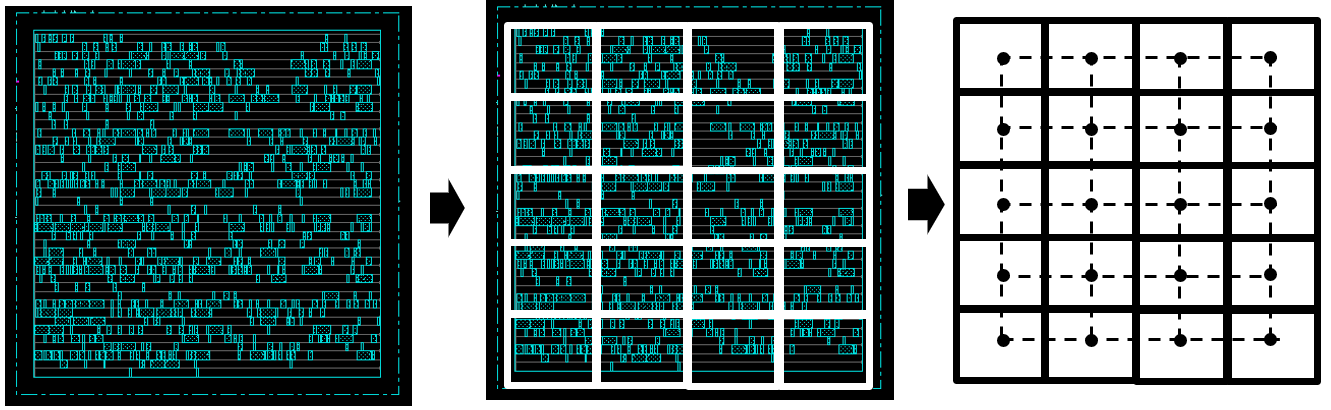
\includegraphics[width=3in]{grid_model}
	\caption{The design is divided into rectangular tiles (solid lines). The dark
		circles and dashed lines represent the vertices and the edges of the grid graph, respectively.}
	\label{fig:grid_model}
\end{figure}

Global routing is performed on a grid which is the logical graph representation of the physical chip. The grid graph \emph{G} is tile-based, which means that the entire chip is partitioned into multiple sub-regions, as illustrated in Fig.~\ref{fig:grid_model}. Each sub-region is referred to as a grid cell, or a global routing cell. The cells are further subdivided with vertical and horizontal gridlines, referred to as routing tracks, along which routes are determined and wires can be created. Each vertex in \emph{G} represents a corresponding tile, and each edge in \emph{G} between vertices corresponds to the shared boundary of two tiles.

\subsection{Routing Metrics}
\subsubsection{Routing Capacity}
The graph \emph{G} used for global routing needs to capture the capacities of the routing regions. The capacity of an edge \emph{e} $\in$ \emph{G} between two vertices \emph{u} and \emph{v} is defined as the maximum number of available routing tracks between the routing regions of \emph{u} and \emph{v}. 

High precision capacity metric can be complex and possible in practice, such track-based capacity can be extended to consider specific routing elements such as blockages, vias and fixed pins. Such elements have different penalties to their respective edge capacity. For example, blockages may consume the capacity of an entire edge. 
\subsubsection{Congestion}
If the total usage of one edge is larger than its capacity, then the tile containing that edge is considered to be congested, with a congestion value defined as $c(e)=\text{usage}(e)/\text{capacity}(e)$. Detailed routing would not be able to route all nets assigned to congested areas due to lack of routing resources. However, there is generally a degree of tolerance as a detailed router may be able to spread the wires from the congested tiles to adjacent less-congested tiles, if those are available.
\subsubsection{Overflow}
Similarly to congestion, when the usage of a tile is greater than its capacity, the amount of overhead is referred to as {\it overflow}, $of(e)=\text{usage}(e)-\text{capacity}(e)$.
% \subsubsection{Wirelength}
% The minimization of wirelength is another important metric for global routing. Decreased wirelength implies smaller power consumption and delays, which are two key factors for  performance-driven optimization. Inherently, congestion minimization conflicts with wirelength minimization, because detours may be introduced to avoid congested regions and that leads to longer wirelength. Therefore, the trade-off between these features has to be carefully tuned based on the requirements of circuit design. 

\subsection{Routability Problem Formulation}
The key objective is to maximize the routability of a design, which is used as a metric to predict the overall quality of routine generated for a  circuit subjected to net and other design constraints.
So the routing problem can be formulated as follows:
\begin{subequations}
\begin{align*}
    \max  \       & f(X), \\
    \text{s.t.}~~ & d(X) \leq 0, \\
                  & n(X) \leq 0,
\end{align*}
\end{subequations}
where f(X) is the measure of quality (routabibility), and $n(X)$ denote network constraints and $d(x)$ denotes a set of other design constraints.  Network constraints indicate that the topology of the network must satisfy certain requirements.  E.g., pins of each net all have to be  connected without loops. Design constraints, on the other hand, are to ensure that the implementation of the network topology meets certain requirements. E.g., that there be no overlapping routes on the same layer or that the routing direction follows a layer's specifications. Our work fits within the routability optimisation problem.

\subsection{Supervised Data Learning Technique}
Data-learning is a powerful technique which can drive knowledge from large amounts of data to predict and generalise unseen data patterns. There are four main categories of data learning: supervised, Unsupervised, semi-supervised, and reinforcement learning. In the research field of physical design algorithms, supervised learning is widely used.

As illustrated in Fig.~\ref{fig:ml_flow}, given certain features as input, the training process builds a set of models which are subsequently evaluated. One way of testing the quality of models is by feeding the same input features as those fed during training to see how closely the predicted values match the the original target output. After such an evaluation, acceptable models are selected for making the predictions in two sets of ML applications. 
\begin{figure}[tb!]
    \centering
    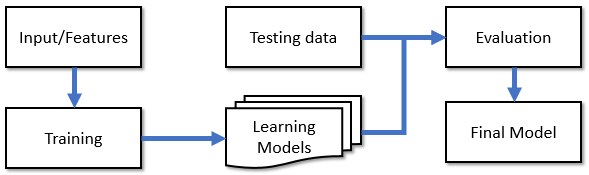
\includegraphics[width=.68\linewidth]{ML_flow}
    \caption{Supervised learning flow.}
    \label{fig:ml_flow}
\end{figure}
There are two types of applications: Regression and classification. {cite a reference and skip the following paragraph} 
\begin{itemize}
\item Regression: Given input to predict continuous values ?????. For example, guess the height of one individual human based on one's age. 
\item Classification. The goal is to predict discrete values. Determine if an email is spam or not, a human is female or male. 
[BAD EXamples.  Use one that is relevant!]
\end{itemize}
